\documentclass[../main.tex]{subfiles}
%!TEX root = ./analysisHighLevelParametrization.tex
\graphicspath {{../}}

\begin{document}
\section{High Level Parametrization} \label{highLevel}
The parametrization of the airship changes depending the users selected main input parameter. In the GUI, there are 3 input parameters: weight, speed, and flight time.

\begin{figure}[H]
	\centering
	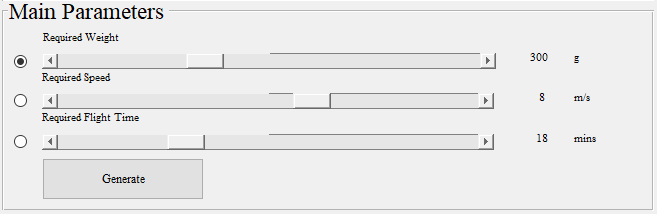
\includegraphics[width=\linewidth]{img/paramaterization/userInputs.PNG}
	\caption{Input parameters in the GUI}
	\label{fig:userInputs}
\end{figure}

The radio button beside the parameters in Figure \ref{fig:userInputs} are meant to signify that the parameter in question is the driving parameter. Based on which parameter is driving, the program will execute and optimize differently. The program will always make the driving parameter its first priority, and  then attempt to get the other two parameters as close to the desired inputs as possible. Failure to reach the driving parameters user input results in a failure. The high level parametrization is therefore split up into 3 parts: weight, speed, and flight time.\\

One important metric used throughout the process is the \textit{badness} of the parameter. The badness of a parameter is a measure of how far away the value of the parameter is from the desired position. It is essentially an error calculation without an absolute value. A positive badness indicates that the parameter is lower than the desired value, while a negative badness value indicates the parameter is better than the desired value.

\subsection{Weight Driven Parametrization}

\begin{figure}[H]
	\centering
	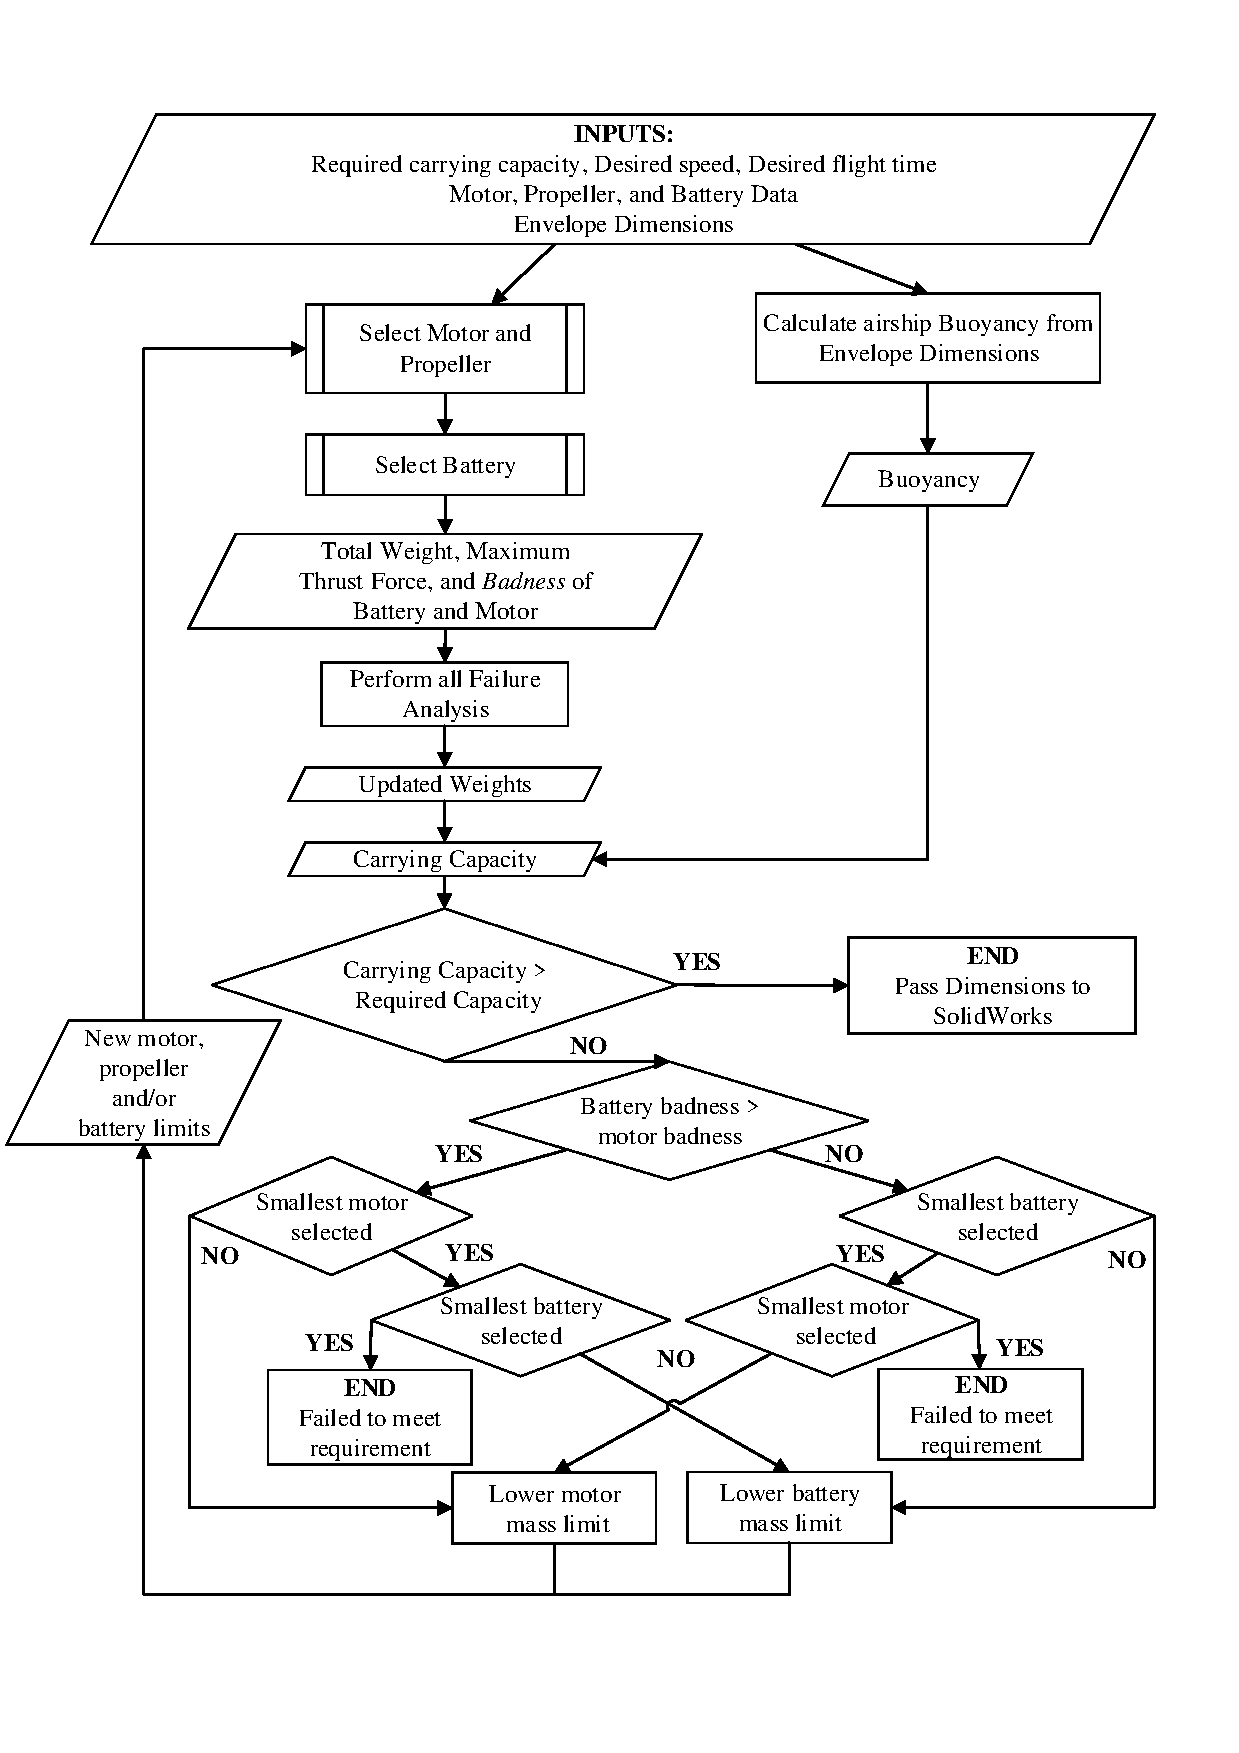
\includegraphics[width=0.95\linewidth]{img/paramaterization/weightBased.pdf}
	\caption{Parametrization Outline For Weight Driven Optimization}
	\label{fig:weightDriven}
\end{figure}

\subsection{Speed Driven Parametrization}

\begin{figure}[H]
	\centering
	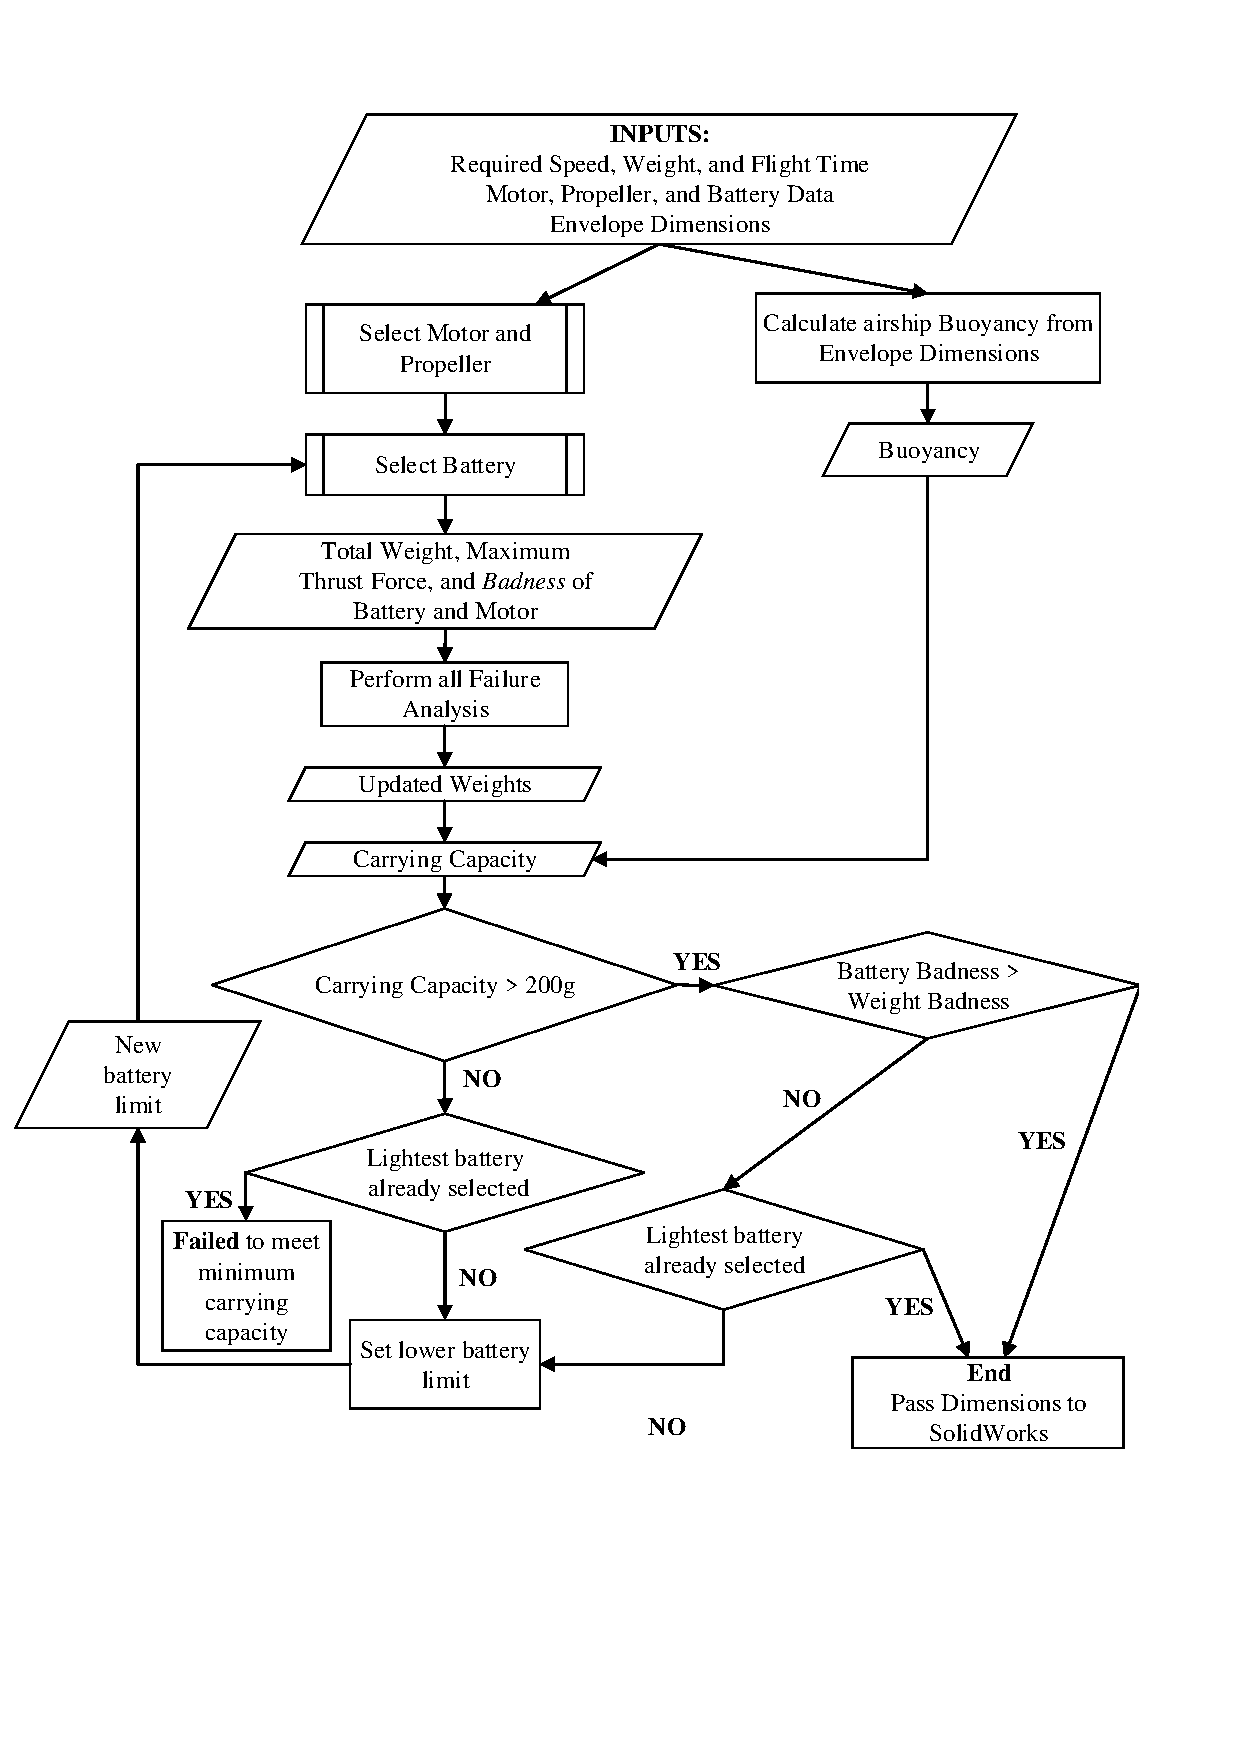
\includegraphics[width=\linewidth]{img/paramaterization/speedBased.pdf}
	\caption{Parametrization Outline For Speed Driven Optimization}
	\label{fig:speedDriven}
\end{figure}


\subsection{Flight-Time Driven Parametrization}

\begin{figure}[H]
	\centering
	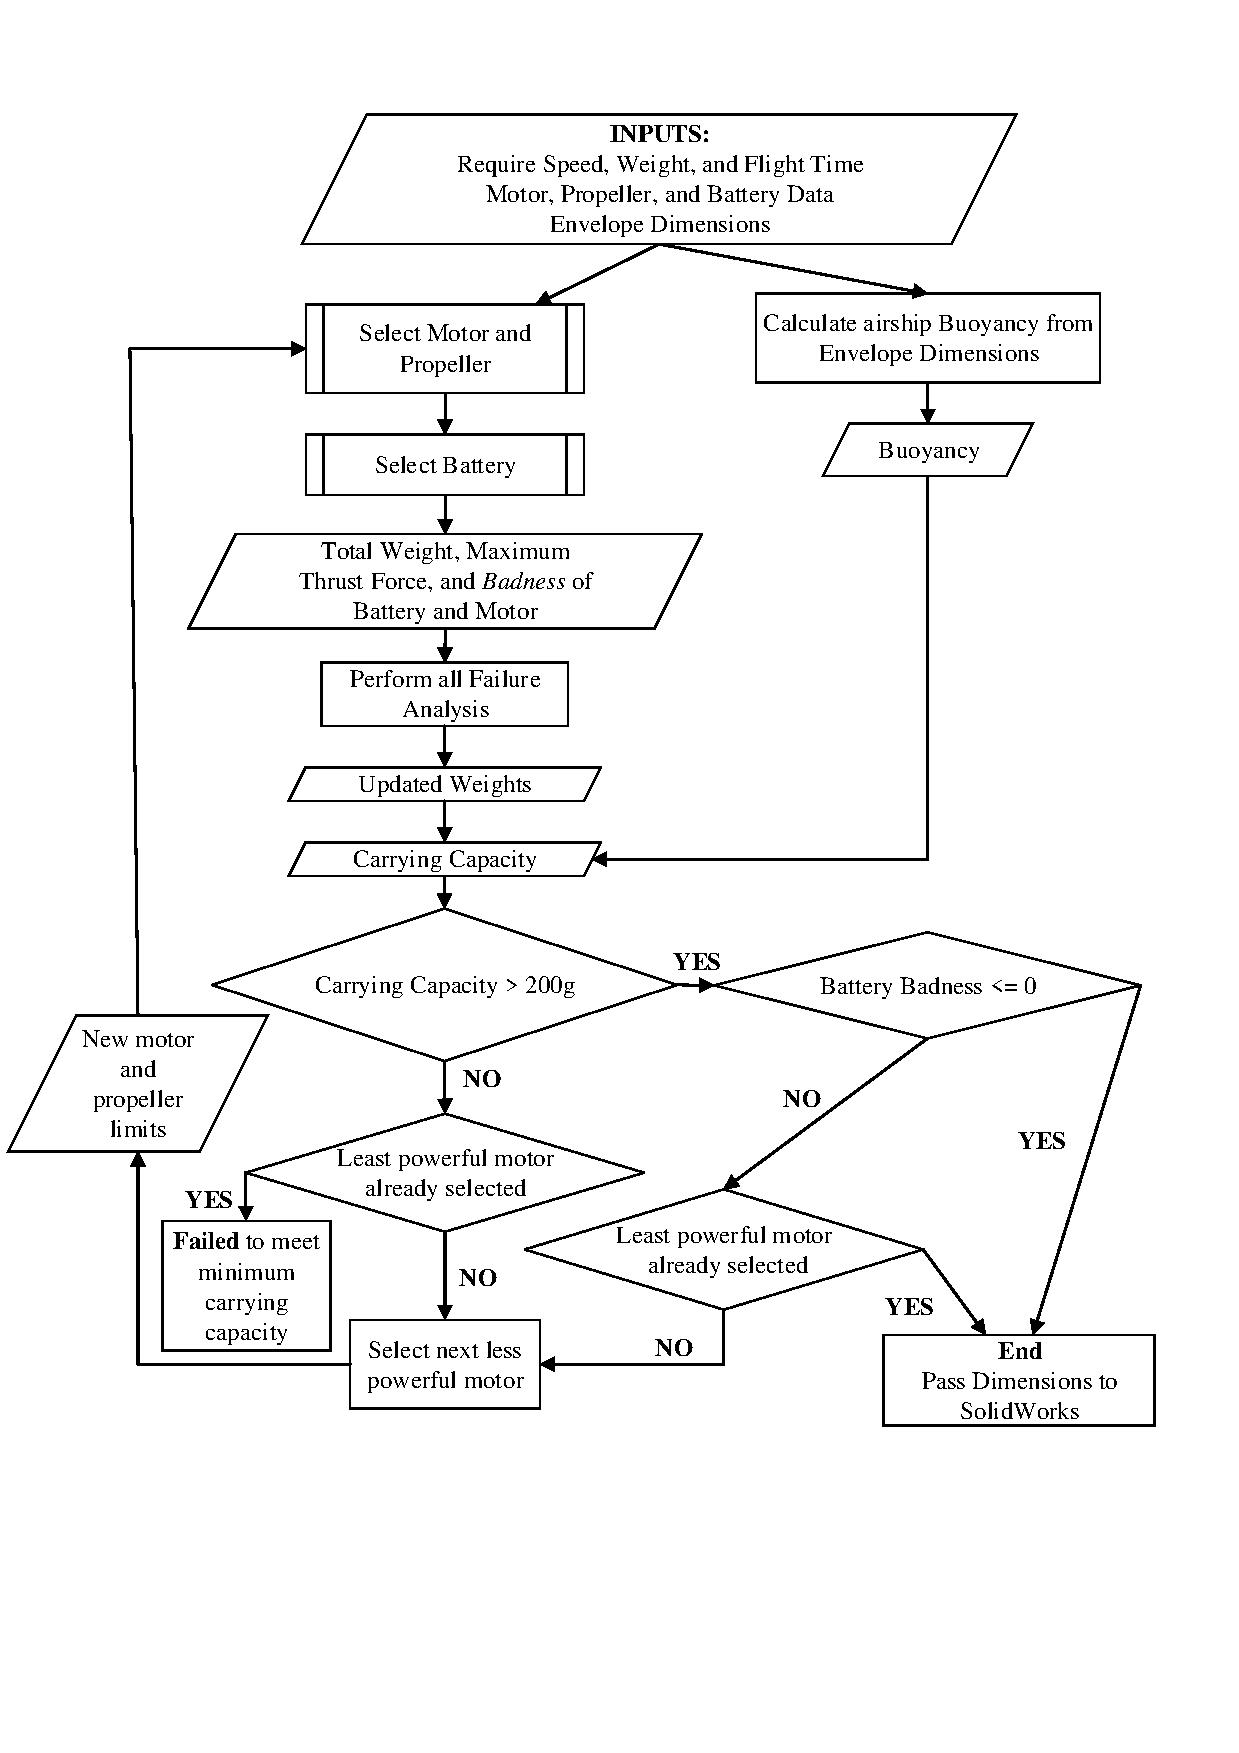
\includegraphics[width=\linewidth]{img/paramaterization/timeBased.pdf}
	\caption{Parametrization Outline For Flight-Time Driven Optimization}
	\label{fig:timeDriven}
\end{figure}

The sub-processes for selecting the motors and propellers are shown in Sections \ref{motorSelect} and \ref{batterySelect}, respectively. The Failure analysis outlines are shown from sections \ref{thrustShaft} to \ref{snapFit}.

\end{document}